% !TeX root = ../paper.tex
\section{Real-Robot Piper Evaluation Details}
\label{appendix:real-robot-piper}

\subsection{Experimental Platform and Configuration}
\label{app:piper-platform}

The real-robot experiments use a bimanual Piper setup. Table~\ref{tab:piper-setup}
summarizes the experimental platform, sensing and control settings, and evaluation scale.

% !TeX root = ../paper.tex
\begin{center}
\begin{minipage}{\linewidth}
\centering
\normalsize
\setlength{\tabcolsep}{3pt}
\renewcommand{\arraystretch}{1.12}
\setlength{\belowcaptionskip}{\baselineskip}
\captionof{table}{Piper real-robot sensing, execution, and evaluation configuration.}\label{tab:piper-setup}
\begin{tabular}{@{}>{\raggedright\arraybackslash}p{0.38\linewidth}>{\raggedright\arraybackslash}p{0.56\linewidth}@{}}
\toprule
Parameter & Configuration \\
\midrule
Robot platform & Bimanual Piper setup \\
RGB acquisition resolution & Main view and two wrist-mounted views, each at $640\times480$ \\
Camera and control frequency & 30~FPS per camera, matched to the robot control frequency \\
Predicted action chunk length & 50 control steps \\
Executed actions per prediction & 25 control steps \\
Task and trial counts & 10 tasks per capability, 20 trials per task \\
Episode budget & 1,000 control steps \\
\bottomrule
\end{tabular}
\end{minipage}
\end{center}
%

\subsection{Task Composition and Trial Arrangement}
\label{app:piper-tasks}

Semantic, Visual Prompt, and Control each contain 10 tasks, with 20 trials per
task, for a total of 600 trials per model.

The representative trajectories below use one task from each category:
folding a towel from bottom to top (Semantic), placing the bowl marked by a
red circle on the shelf (Visual Prompt), and changing the Control instruction
during execution from placing a sticker on top of a box to placing it on
the front. 

\subsection{Representative Execution Trajectories}
\label{app:piper-trajectories}

Each category is illustrated by one representative execution video. Frames
within each contact sheet are ordered from left to right and then from top
to bottom, providing a compact summary of the corresponding behavior.

% Keep the three equally sized real-robot sequences on one page.
% !TeX root = ../paper.tex
\begin{figure}[!htbp]
\centering
\setlength{\parskip}{0pt}
\setlength{\abovecaptionskip}{\baselineskip}
\setlength{\belowcaptionskip}{0pt}
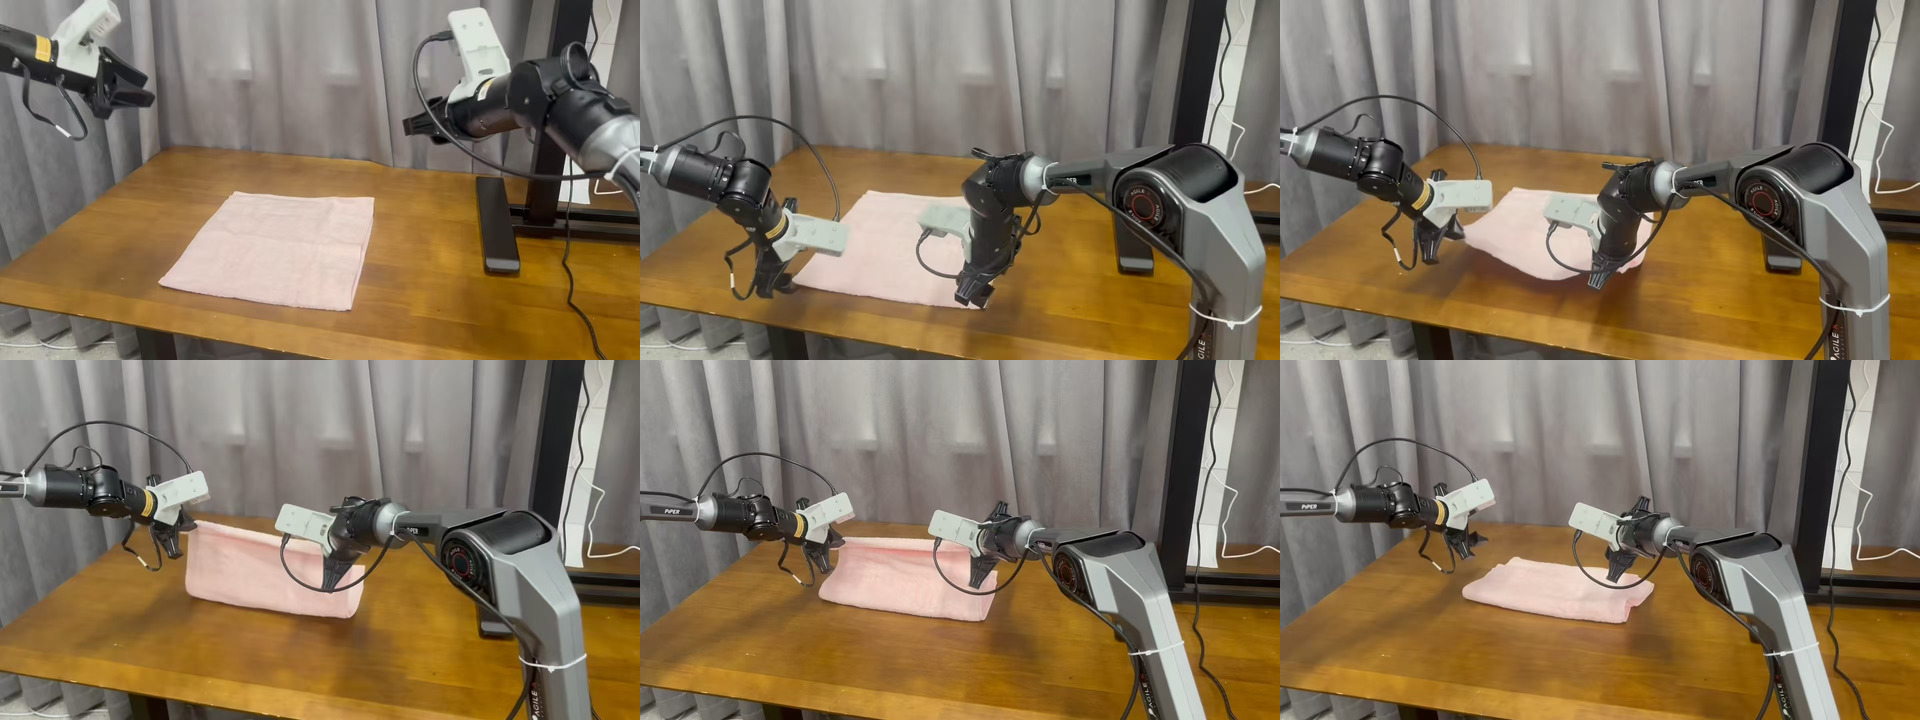
\includegraphics[width=.95\linewidth]{figures/piper_trajectories/towel_contact_sheet.jpg}\par\nointerlineskip
\caption{Piper Semantic task execution. Task instruction: ``Fold the towel from bottom to top.''}
\label{fig:piper-semantic-trajectory}
\par\vspace{\baselineskip}\nointerlineskip
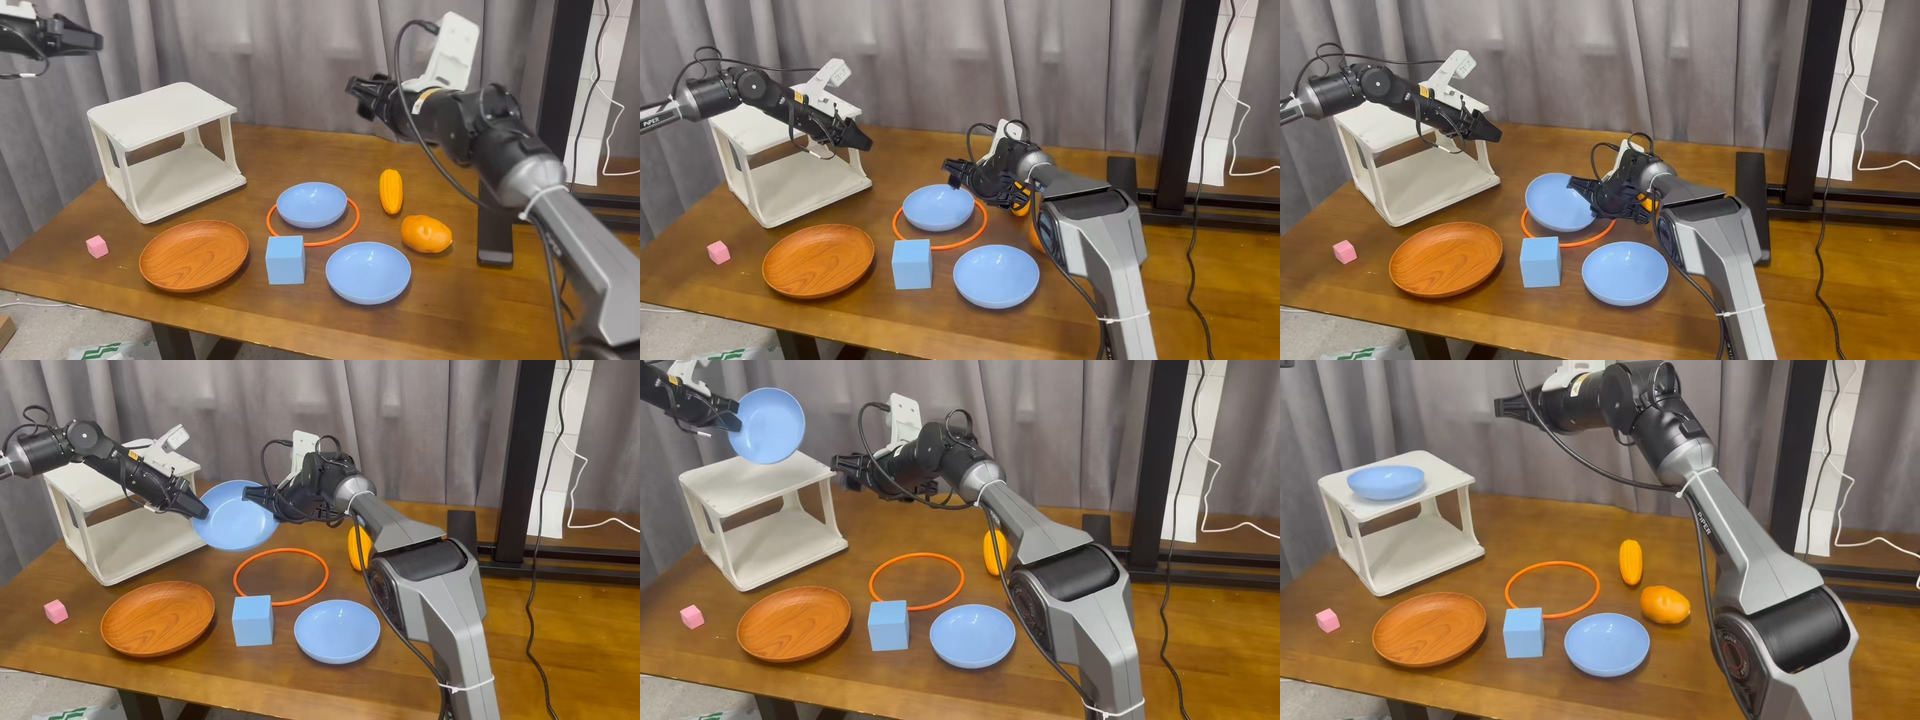
\includegraphics[width=.95\linewidth]{figures/piper_trajectories/spatial_contact_sheet.jpg}\par\nointerlineskip
\caption{Piper Visual Prompt task execution. Task instruction: ``Place the bowl marked by the red circle on the shelf.''}
\label{fig:piper-vis-trajectory}
\par\vspace{\baselineskip}\nointerlineskip
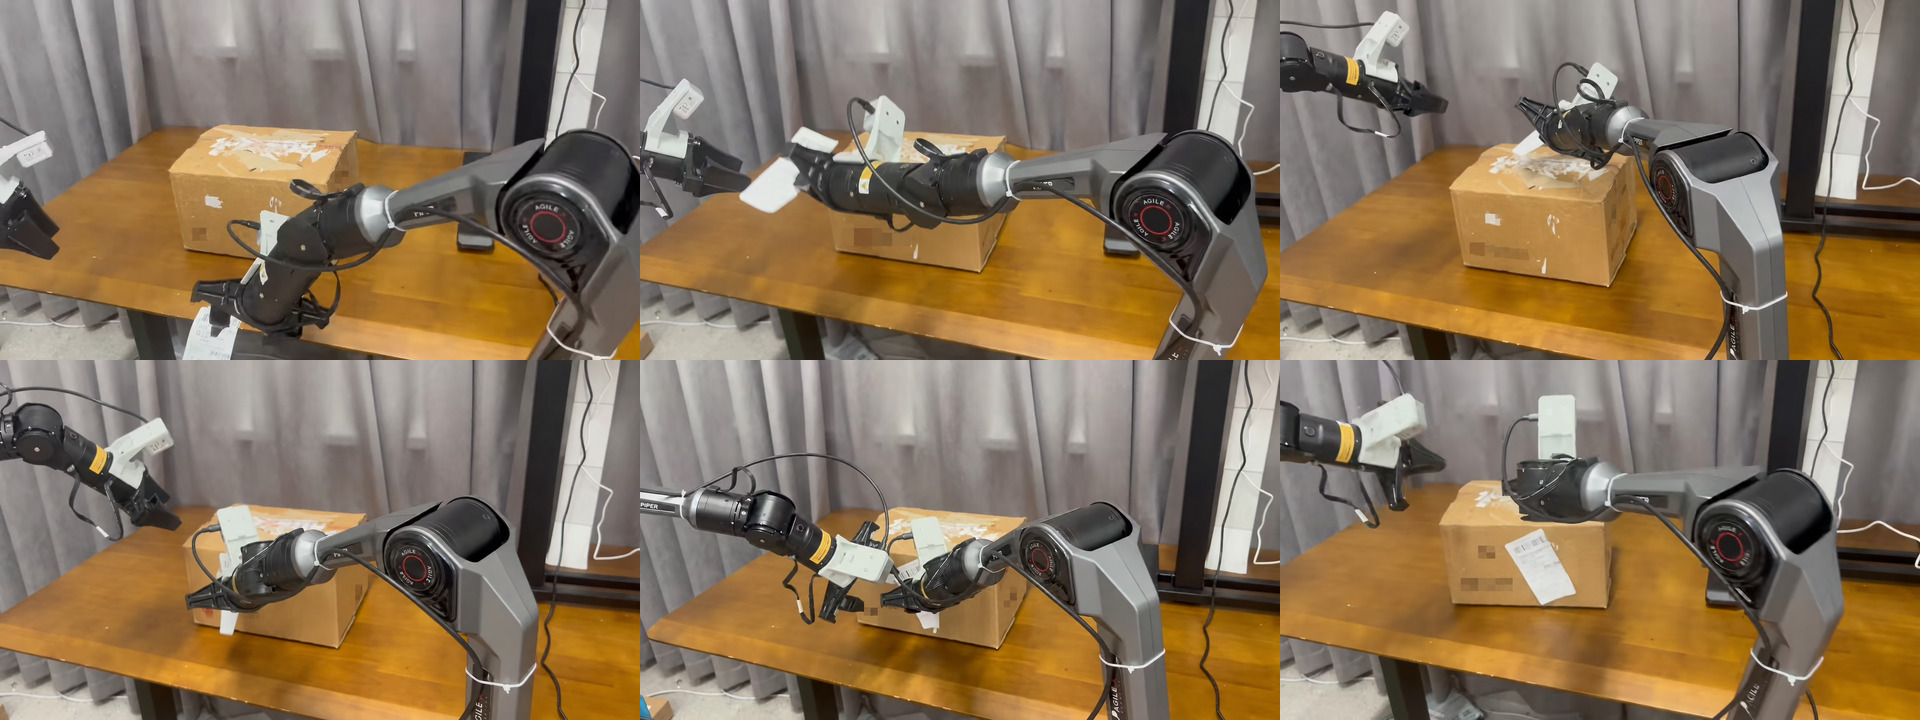
\includegraphics[width=.95\linewidth]{figures/piper_trajectories/control_contact_sheet.jpg}\par\nointerlineskip
\caption{Piper Control task execution. The initial instruction, ``Attach the sticker to the top of the box,'' is replaced during execution by ``Attach the sticker to the front of the box.''}
\label{fig:piper-control-trajectory}
\end{figure}
%

